\newpage
\section{Introduzione}
\subsection{Descrizione del progetto}
%L’equalizzazione di un’immagine prevede l’aumento del contrasto tramite il ripristino dei punti più chiari e più scuri, nonché la successiva distribuzione uniforme dei valori su questi due tipi di punto. 
Lo scopo del progetto é quello di realizzare un equalizzatore di immagini in bianco e nero, ovvero un componente che permetta di ricalibrare il contrasto al fine di incrementarlo.

Questa operazione viene effettuata modificando i valori di intensitá dei singoli pixel (i quali assumono un valore compreso tra 0 e 255 che indica la quantitá di bianco presente) per redistribuire in maniera piú equa la composizione dell'istogramma\footnote{Istogramma: rappresenta la distribuzione dei pixel chiari (sulla porzione di destra) e scuri (sulla sinistra) dell'immagine} (come mostrato in Figura \ref{istogramma}).



%immagine
\begin{figure}[ht]
    \centering       
    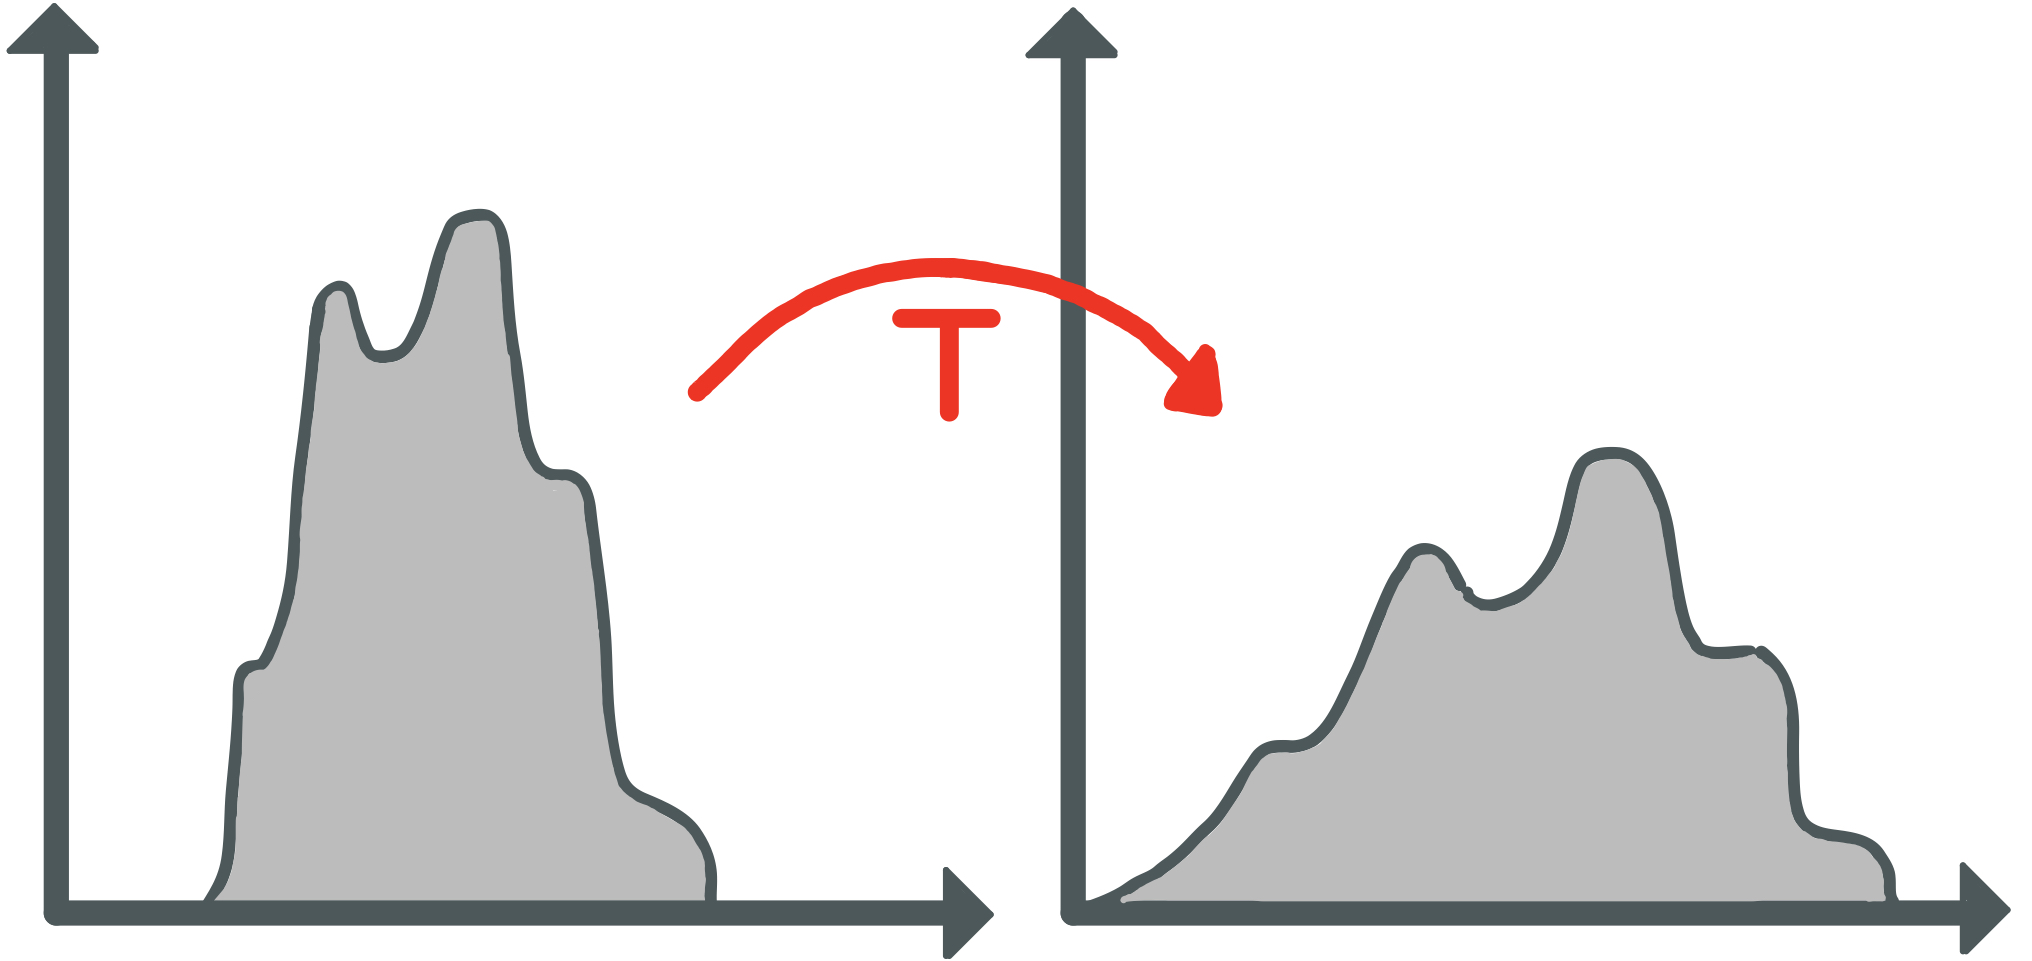
\includegraphics[scale = 0.08]{Figure/istogramma} %tra le graffe mettere il nome del file che va importato qui di fianco, sotto il main.tex
    \caption{Trasformazione dovuta all'equalizzazione}
    \label{istogramma}
\end{figure}

\subsection{Specifiche generali}
L'immagine è letta sequenzialmente da memoria, dove si trova memorizzata come mostrato in Figura \ref{elaboratore}. %In questa fase vengono calcolati dall'elaboratore i valori massimo e minimo di intensitá dei pixel che saranno poi utilizzati nella fase successiva.
Ogni pixel dell'immagine è trasformato per mezzo dell'algoritmo fornito e riscritto in memoria a partire dalla prima cella disponibile.

%piccolo esempio
Un esempio di funzionamento del componente è mostrato in Figura \ref{elaboratore} dove il blocco "Elaboratore" è quello realizzato dalla entity \texttt{"project\_reti\_logiche"}.
%In figura é possibile distinguere 3 tipologie differenti di frecce, alcune entranti nella macchina e altre uscenti. Le prime (frecce rosse) stanno ad indicare il flusso di dati in ingresso al componente una volta che quest'ultimo richiede alla memoria il contenuto di uno specifico indirizzo. Le frecce in blu rappresentano il flusso di dati in uscita dal componente una volta terminata la fase di modifica del pixel, questi vengono salvati in memoria specificando l'indirizzo nel quale si desidera memorizzare il dato. Infine la freccia nera consente di interagire con la memoria, in lettura e scrittura, andando a specificare di quale indirizzo si desidera sapere il contenuto o andare a memorizzare informazioni.
Il modulo comunica alla memoria gli indirizzi da cui vuole leggere o su cui vuole scrivere (freccia nera), legge il valore dei pixel (frecce rosse), applica l'algoritmo e scrive in uscita i valori sulla memoria (frecce blu).

L’indirizzo x rappresenta il primo indirizzo di memoria nel quale si andrá a memorizzare l’immagine.


%immagine
\begin{figure}[ht]
    \centering           %0.3
    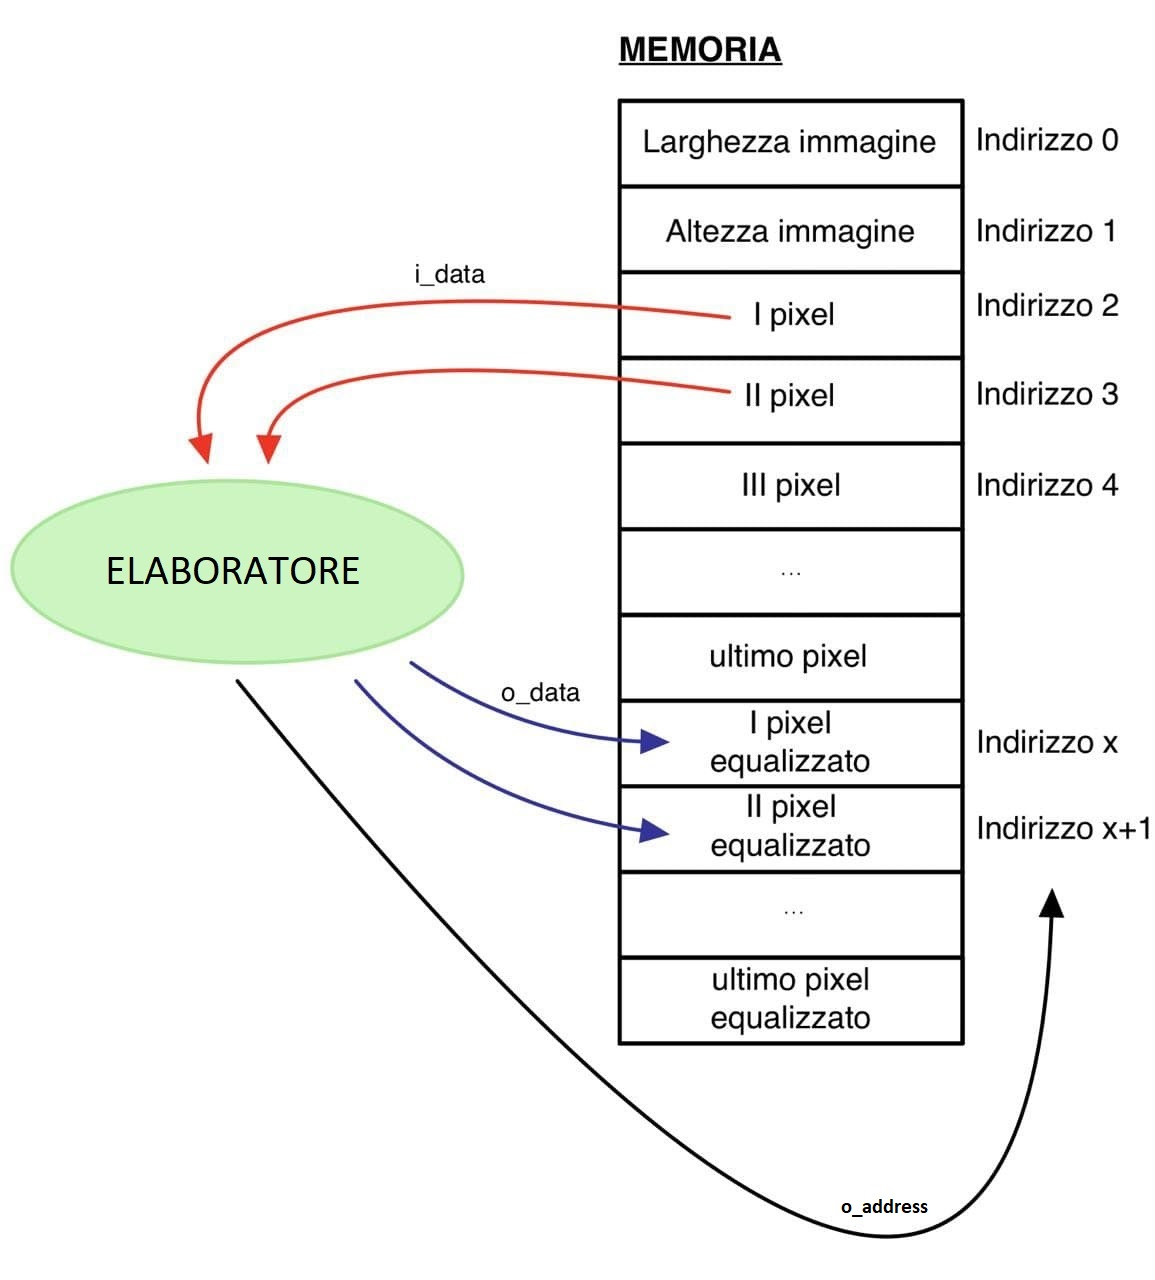
\includegraphics[scale = 0.205]{Figure/elaboratore} %tra le graffe mettere il nome del file che va importato qui di fianco, sotto il main.tex
    \caption{Funzionamento ad alto livello del componente (Elaboratore)}
    \label{elaboratore}
\end{figure}

\clearpage